%%%%%%%%%%%%%%%%%%%%%%%%%%%%%%%%%%%%%%%%%%%%%%%%%%%%%%%%%%%%%%%%%%% 
%                                                                 %
%                            CHAPTER                              %
%                                                                 %
%%%%%%%%%%%%%%%%%%%%%%%%%%%%%%%%%%%%%%%%%%%%%%%%%%%%%%%%%%%%%%%%%%% 

\chapter{Inleiding}

\section{Situering}
Sociale media is zo goed als niet meer weg te denken uit het huidige moderne
leven. Over de jaren heen zijn er verschillende definities gegeven. In het werk
van Howard en Park wordt sociale media gedefinieerd als de infrastructuur en
tools om content te maken en te verspreiden\cite{PhilipsAndParks}. Deze
definitie is erg ruim, en vertakt zich dus in heel wat facetten, waaronder
sociale netwerken, media sharing networks, etc. Maar ook de fitnesstrackers.
Deze opkomst van nieuwe media brengt echter ook onbedoelde maar significante
privacy bezorgdheden met zich mee.

De focus in deze dissertatie ligt op privacy binnen fitnesstrackers, meer
specifiek platformen die \ac{gps}-locaties gebruiken, zoals Strava, Nike Run
Club, etc. Dit zijn platformen waar personen sportactiviteiten zoals lopen,
fietsen, wandelen,\ldots kunnen delen met elkaar. Het algemene concept is
hierbij dat wanneer je een sportactiviteit uitvoert, je deze voor je volgers en
vrienden beschikbaar maakt. De sportactiviteiten zullen natuurlijk bepaalde
gegevens bevatten die zichtbaar zijn voor die andere gebruikers,
Figuur~\ref{fig:activityExample} geeft bijvoorbeeld weer hoe Strava de afstand,
bewegingstijd, en natuurlijk de \ac{gps}-locaties deelt. Vele van deze gegevens
hebben direct of indirect een negatieve impact op de privacy van de user. Deze
negatieve gevolgen komen dan vooral in de vorm van het onbedoeld vrijgeven van
\textit{gevoelige locaties}. Onder het concept van een gevoelige locatie vallen
\textit{gevoelige locaties}. Onder het concept van een gevoelige locatie vallen
heel wat beschrijvingen. Een algemene beschrijving kan zijn, een locatie die
geografische informatie deelt die negatieve gevolgen kan hebben, en die je dus
liever niet deelt. In het kader van dit onderzoek zal dit gaan over start en
eindlocaties van activiteiten. Dit kan gaan over woonplaatsen, wat kan leiden
tot o.a.\ stalking. Alsook locaties waar sportmateriaal wordt opgeborgen. Er
zijn gevallen bekend van fietsdieven die Strava gebruiken om fietsen te kunnen
lokaliseren\cite{Sportapp72:online}\cite{Cyclistw89:online}. Grootschaligere
voorbeelden die zeker het vermelden waard zijn, zijn de gevallen waarbij
geheime militaire basissen ontdekt worden door het bestuderen van de
heatmap\cite{Fitnesst33:online}.
\begin{figure}
    \centering
    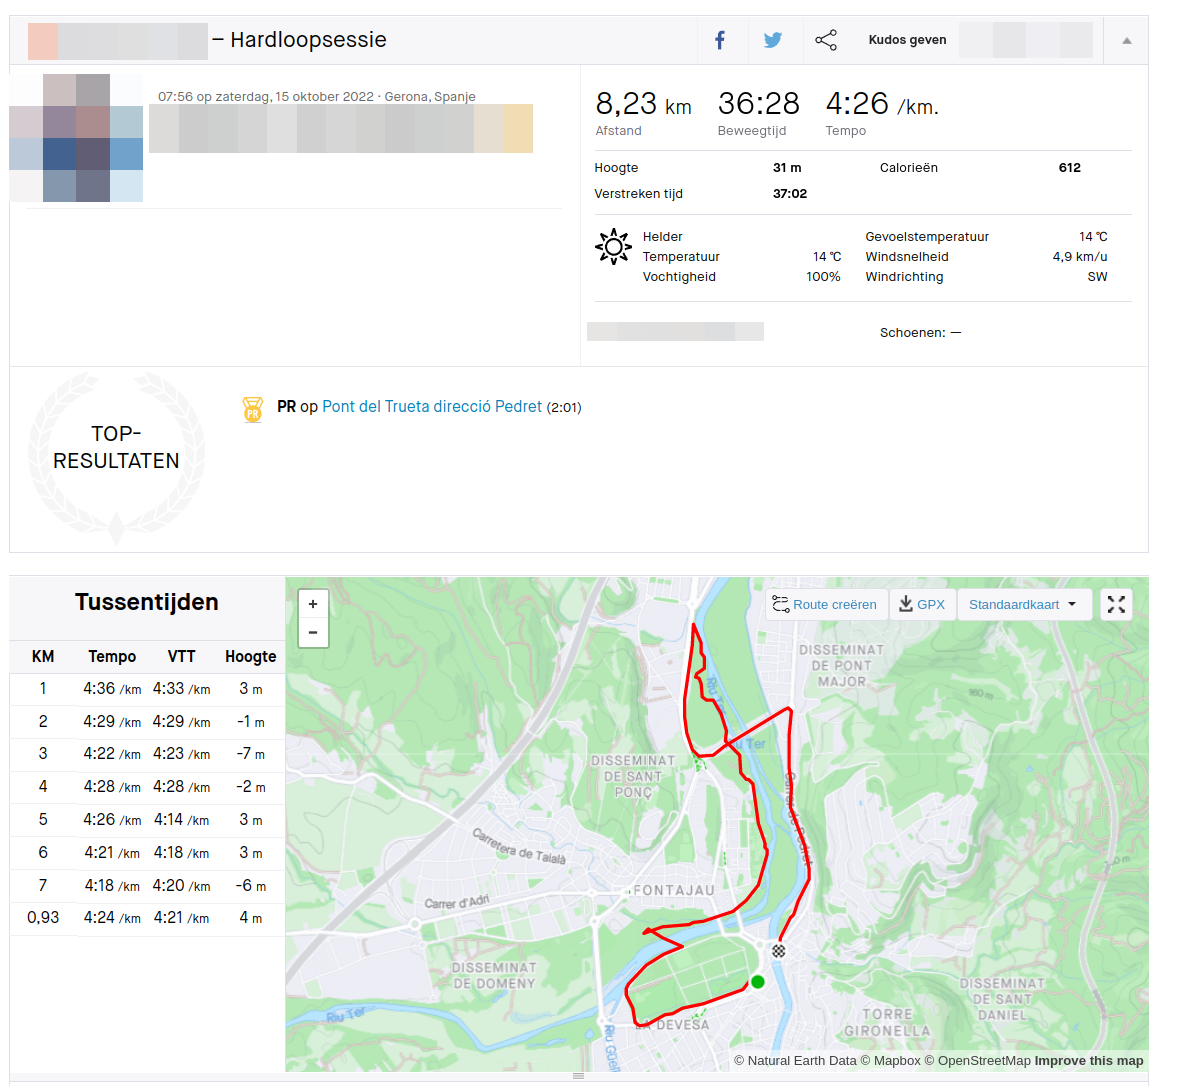
\includegraphics[width=0.5\linewidth]{fig/VoorbeeldActiviteiten/VoorbeeldActiviteit_Cropped.png}
    \caption{Voorbeeldactiviteit Strava}\label{fig:activityExample}
\end{figure}

Deze platformen implementeren elk manieren om de privacy van de users te
verbeteren. De meest eenvoudige te bedenken is misschien wel de mogelijkheid om
activiteiten te verbergen voor een selectie van personen (bv.\ iedereen die
geen volger is). Zo kunnen enkel de mensen die de gebruiker expliciet toelaat
activiteiten bekijken. Een complexer alternatief is het gebruik van \acp{EPZ}.
Hierbij wordt de weergegeven route voor de persoon die meekijkt gedeeltelijk
verborgen. Er wordt als het ware een deel van de route afgekapt. De echte
begin- en eindpunten zullen binnenin het afgekapte deel liggen. Er zullen
nieuwe punten worden gegenereerd, op de rand van de cirkel, die voor de externe
waarnemer het begin en einde zullen voorstellen. Het begin- en eind-deel van de
route wordt dus onzichtbaar voor de andere gebruikers. Door de aanwezigheid van
al deze pogingen tot privacyverbeteringen valt op dat de ontwikkelaars van de
platformen erg bewust zijn van de mogelijke gevaren. Echter is er een afweging
te maken bij de implementatie tussen de bruikbaarheid van het platform, en de
privacy van de eindgebruiker. Hoe meer data wordt vrijgegeven, hoe groter de
kans op mogelijk gevoelige info wordt meegegeven. Aan de andere kant, bij het
weglaten van informatie gaat de gebruiksvriendelijkheid en de aanwezigheid van
nuttige data van het platform serieus achteruit.

\section{Doelstelling}
In dit onderzoek bekijken we of er een mogelijkheid bestaat om private locaties
(verborgen start- en eindlocaties) van een activiteiten te achterhalen, ondanks
het gebruik van de \ac{EPZ}~\ref{EPZ} als privacy beveiligingsmechanisme. In
het verleden werden enkele manieren beschreven om a.d.h.v.\ andere metadata
zoals hoogtedata en afstanden de \ac{EPZ} te omzeilen
(\textit{\cite{Dhondt_Pochat_Voulimeneas_Joosen_Volckaert_2022},\cite{Verdonck_2022}}).
Gedurende deze thesis wordt meer in detail gegaan op het gebruik van
snelheidsdata. Als basis voor deze aanval wordt de inferentie aanval op de EPZ
van~\citeauthor{Dhondt_Pochat_Voulimeneas_Joosen_Volckaert_2022} genomen. Er
wordt dan onderzocht of deze aanval nog steeds mogelijk is bij het weglaten van
bepaalde gegevens, en dus door het gebruik van andere gegevens. De focus ligt
in deze studie voornamelijk op snelheidsdata.

Om deze doelstelling te bekomen is eerst een berekeningsmechanisme nodig voor
de afstanden die nodig zijn om de inferentie-aanval te kunnen uitvoeren. Daarna
moet een analyse uitgevoerd worden tussen de berekende afstanden, en de waarden
afgeleid volgens de berekeningen
van~\citeauthor{Dhondt_Pochat_Voulimeneas_Joosen_Volckaert_2022}. Zo kan de
effectiviteit van de aanval a priori worden geschat. Er is een analyse van de
beschikbare data, en een bespreking en reflectie over de resultaten van de
aanval.